\section{LEVEL 5 · Samenhang versus causaliteit}

\begin{missie}
Missie: ontdek wanneer ‘het één hoort bij het ander’ ook echt ‘het één veroorzaakt het ander’ betekent. (LPD 12)
\end{missie}

\begin{doel}
\textbf{DOEL} \quad Na dit level kan je:

☐ het verschil uitleggen tussen \textbf{samenhang} en \textbf{causaliteit};

☐ drie misvattingen herkennen: \textbf{omgekeerde oorzakelijke richting}, \textbf{toevallige samenhang} en een \textbf{derde variabele};

☐ \textbf{observationeel} en \textbf{experimenteel} onderzoek onderscheiden;

☐ afleiden of de \textbf{opzet} van een onderzoek causaliteit toelaat, en percentages uit een experiment berekenen en interpreteren.
\end{doel}

\subsection*{Theorie 5.1 · Samenhang is nog geen causaliteit}

\begin{theorie}
\begin{itemize}
\item \textbf{Samenhang} is het statistische verband tussen twee variabelen: ze veranderen samen. Bij twee kwantitatieve variabelen spreken we ook van \textbf{correlatie}.
\item Een \textbf{causaal} (oorzakelijk) verband betekent dat de ene variabele (de \emph{oorzaak}, onafhankelijke variabele $x$) de andere (het \emph{gevolg}, afhankelijke variabele $y$) rechtstreeks beïnvloedt.
\item Is er causaliteit, dan is er zeker samenhang. Is er samenhang, dan is er \textbf{niet zeker} causaliteit.
\end{itemize}
\end{theorie}

\begin{voorbeeld}
\textbf{Voorbeeld.} Hoe meer reddingsacties de redders aan de kust uitvoeren, hoe meer zonnecrème er wordt verkocht. Er is samenhang, maar de zonnecrème veroorzaakt geen reddingsacties. Beide worden beïnvloed door het warme weer.
\end{voorbeeld}

\subsection*{Theorie 5.2 · Drie misvattingen}

\begin{center}
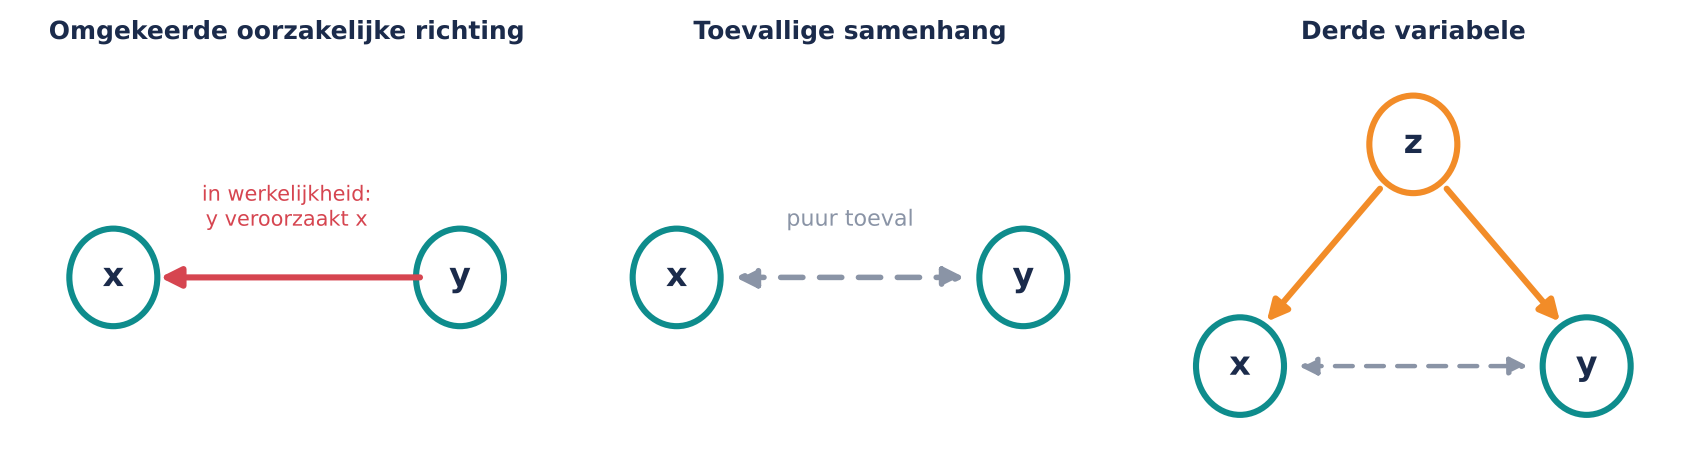
\includegraphics[width=0.95\textwidth]{figuren/d1_misvattingen.png}
\end{center}

\begin{theorie}
\begin{itemize}
\item \textbf{Omgekeerde oorzakelijke richting}: oorzaak en gevolg zijn omgewisseld. \emph{Voorbeeld:} hoe bruiner Dries’ huid, hoe meer zon er scheen. De zon is de oorzaak, de bruine huid het gevolg.
\item \textbf{Toevallige samenhang}: de correlatie berust op louter toeval. Hoe meer verbanden je onderzoekt, hoe groter de kans dat er toevallig een gevonden wordt. \emph{Voorbeeld:} er is in de Verenigde Staten een duidelijke samenhang tussen de kaasconsumptie en het aantal doctoraten in burgerlijke bouwkunde. Kaas heeft niets met doctoraten te maken.
\item \textbf{Derde variabele}: een verborgen variabele $z$ beïnvloedt zowel $x$ als $y$. \emph{Voorbeeld:} wie meer alcohol drinkt, heeft meer risico op longkanker, maar mensen die meer drinken, roken ook meer. Roken is de derde variabele.
\end{itemize}
\end{theorie}

\subsection*{Theorie 5.3 · Observationeel of experimenteel onderzoek}

\begin{theorie}
\begin{itemize}
\item Bij \textbf{observationeel} onderzoek verzamelt de onderzoeker data maar grijpt hij niet in. Een gevonden verband is niet noodzakelijk causaal: andere factoren kunnen meespelen.
\item Bij \textbf{experimenteel} onderzoek grijpt de onderzoeker wel in en bepaalt hij wat er gebeurt. Bij een experimenteel vergelijkend onderzoek worden de deelnemers \textbf{willekeurig} (randomisatie) in twee groepen verdeeld: een \textbf{experimentele groep} (krijgt de behandeling) en een \textbf{controlegroep}. Zo kan je wel een causaal verband vaststellen.
\end{itemize}
\end{theorie}

\begin{voorbeeld}
\textbf{Voorbeeld.} Een trainer vermoedt dat een bepaalde opwarming tot betere looptijden leidt.

\emph{Observationeel:} hij noteert de opwarming en de looptijden die atleten zelf kiezen en vindt samenhang. Mogelijk spelen ook het tijdstip of de ondergrond mee.

\emph{Experimenteel:} hij verdeelt de atleten door loting in twee groepen met een andere opwarming en laat ze op hetzelfde moment hetzelfde parcours lopen. Doet de experimentele groep duidelijk beter, dan is de opwarming de oorzaak.
\end{voorbeeld}

\subsection*{Aan de slag}

\subsubsection*{Oefening 5.1 \quad ★☆☆ \quad Invullen}

\textbf{Woordenlijst:} samenhang – causaliteit – controlegroep – willekeurig – observationeel – experimenteel.

Een statistisch verband tussen twee variabelen heet \gat{samenhang}. Als de ene variabele de andere rechtstreeks beïnvloedt, spreken we van \gat{causaliteit}. Bij \gat{observationeel} onderzoek grijpt de onderzoeker niet in. Bij \gat{experimenteel} onderzoek worden de deelnemers \gat{willekeurig} verdeeld in een experimentele groep en een \gat{controlegroep}.

\subsubsection*{Oefening 5.2 \quad ★★☆ \quad Welke misvatting?}

Kies bij elke uitspraak: \textbf{O} (omgekeerde richting), \textbf{T} (toeval) of \textbf{D} (derde variabele) en leg uit.

\breedtes{52/10/38}
\begin{tabular}{lll}
\hline
Uitspraak & O / T / D & Uitleg \\
\hline
a) Als je veel paraplu’s ziet, regent het. Paraplu’s brengen dus regen. & & \\
b) Kinderen met een grotere woordenschat hebben een grotere schoenmaat. & & \\
c) Het aantal verkochte ijsjes en het aantal zonnebrandgevallen stijgen samen. & & \\
d) Jongeren die veel naar de huisarts gaan, zijn vaker ziek. Huisartsen maken dus ziek. & & \\
e) Het aantal piratenbendes daalde en de gemiddelde temperatuur steeg: piraten houden de aarde koel. & & \\
\hline
\end{tabular}

\begin{oplossing}
\textbf{Oplossing 5.2} \quad a) O: de regen is de oorzaak, paraplu’s het gevolg. b) D: leeftijd (oudere kinderen kennen meer woorden en hebben grotere voeten). c) D: warm weer. d) O: wie ziek is, gaat naar de huisarts. e) T: twee tendensen over de tijd die toevallig samenlopen (geen verband).
\end{oplossing}

\subsubsection*{Oefening 5.3 \quad ★★☆ \quad Context: de natuur en geluk}

Een Europese studie bij 26\,000 mensen toont een positief verband tussen de levenstevredenheid en het aantal vogelsoorten in de buurt. Welke bewering is correct? Verklaar.

\textbf{A} Uit dit observationeel onderzoek blijkt dat de natuur ervoor zorgt dat mensen gelukkiger worden.

\textbf{B} Uit dit observationeel onderzoek blijkt dat gelukkige mensen verhuizen naar plekken met veel vogels.

\textbf{C} Uit dit observationeel onderzoek kan je geen oorzakelijk verband afleiden; daarvoor is een experiment nodig waarbij mensen willekeurig aan leefomgevingen worden toegewezen.

\lijn

\begin{oplossing}
\textbf{Oplossing 5.3} \quad C. Het is observationeel: samenhang is aangetoond, causaliteit niet. A en B zijn allebei een mogelijke, maar niet bewezen, richting van oorzaak en gevolg; er kan ook een derde variabele zijn (bv. inkomen, gezondheid).
\end{oplossing}

\subsubsection*{Oefening 5.4 \quad ★★☆ \quad Experiment: een slaapprogramma}

Een school wil weten of een ‘slaapprogramma’ de slaap van jongeren verbetert. Er worden 400 jongeren \textbf{door loting} verdeeld in een experimentele groep (200, met het programma) en een controlegroep (200, zonder). Na acht weken geven ze aan of ze beter, evenveel of slechter slapen.

\breedtes{28/18/18/18/18}
\begin{tabular}{lcccc}
\hline
 & beter & evenveel & slechter & totaal \\
\hline
experimentele groep & 120 & 60 & 20 & \\
controlegroep & 70 & 100 & 30 & \\
totaal & & & & \\
\hline
\end{tabular}

\textbf{a)} Is dit een experimenteel of een observationeel onderzoek? Waar speelt randomisatie een rol? \lijn

\textbf{b)} Vul de tabel aan. \lijn

\textbf{c)} Bereken met ICT (op 0,1 \% nauwkeurig): welk percentage van de experimentele groep slaapt beter? En van de controlegroep? \lijn

\textbf{d)} Welk percentage van de jongeren die slechter slapen, zat in de controlegroep? \lijn

\textbf{e)} Interpreteer de resultaten. Mag je besluiten dat het programma de slaap verbetert? Verklaar. \lijn

\begin{oplossing}
\textbf{Oplossing 5.4} \quad a) Experimenteel (de onderzoekers grijpen in); randomisatie bij het verdelen van de jongeren in de twee groepen door loting. b) Totalen rij 1: 200; rij 2: 200; totaal: 190 – 160 – 50 – 400. c) $\frac{120}{200}=60{,}0\,\%$ en $\frac{70}{200}=35{,}0\,\%$. d) $\frac{30}{50}=60{,}0\,\%$. e) In de experimentele groep slaapt een veel groter deel beter (60 \% tegenover 35 \%). Doordat de groepen door loting zijn gevormd, is het verschil waarschijnlijk te wijten aan het programma: causaliteit is hier mogelijk.
\end{oplossing}

\subsubsection*{Oefening 5.5 \quad ★★★ \quad Een experiment ontwerpen}

Een kinderopvang wil weten of een dagelijks voorleesmoment de woordenschat van kleuters vergroot.

\textbf{a)} Waarom is een observationeel onderzoek (kinderen vergelijken die thuis al veel of weinig worden voorgelezen) niet geschikt om causaliteit aan te tonen? Noem een derde variabele. \lijn

\textbf{b)} Beschrijf een experiment: wie zit in welke groep, hoe verdeel je ze en wat meet je? \lijn

\textbf{c)} Waarom moeten beide groepen in dezelfde omstandigheden verblijven (behalve het voorleesmoment)? \lijn

\begin{oplossing}
\textbf{Oplossing 5.5} \quad a) Ouders die veel voorlezen hebben bijvoorbeeld ook een hoger opleidingsniveau of praten meer met hun kind; die derde variabele kan de woordenschat verklaren. b) Kleuters worden door loting verdeeld in een experimentele groep (dagelijks voorlezen) en een controlegroep (geen extra voorleesmoment); na enkele maanden meet men de woordenschat in beide groepen met dezelfde test en vergelijkt men gemiddelden. c) Zo komt een verschil enkel door het voorleesmoment en niet door andere factoren.
\end{oplossing}

\subsection*{Koppel · begrip en omschrijving}

\breedtes{34/66}
\begin{tabular}{ll}
\hline
Begrip & Omschrijving \\
\hline
1. samenhang & A. De onderzoeker grijpt in en bepaalt wie de behandeling krijgt. \\
2. causaliteit & B. Statistisch verband tussen twee variabelen. \\
3. derde variabele & C. Een verborgen variabele beïnvloedt beide onderzochte variabelen. \\
4. experimenteel onderzoek & D. De ene variabele beïnvloedt rechtstreeks de andere. \\
5. controlegroep & E. De groep die de behandeling niet krijgt en dient als vergelijking. \\
\hline
\end{tabular}

Mijn antwoord: 1 – \_\_\quad 2 – \_\_\quad 3 – \_\_\quad 4 – \_\_\quad 5 – \_\_

\begin{oplossing}
\textbf{Oplossing Koppel} \quad 1 – B \quad 2 – D \quad 3 – C \quad 4 – A \quad 5 – E
\end{oplossing}

\subsection*{Foutjager}

\textbf{1.} Mo: ‘Er is een sterke correlatie tussen gamen en slechte punten, dus gamen veroorzaakt slechte punten.’ \lijn

\textbf{2.} Lies: ‘In een experiment laat ik de vrijwilligers in de testgroep en de rest in de controlegroep.’ \lijn

\textbf{3.} Kobe: ‘Als er geen samenhang is, kan er toch een causaal verband zijn.’ \lijn

\begin{oplossing}
\textbf{Oplossing Foutjager} \quad 1. Samenhang bewijst geen oorzaak: omgekeerde richting (wie slechte punten heeft, speelt meer) of een derde variabele (bv. weinig motivatie). 2. De groepen moeten willekeurig worden samengesteld (randomisatie), anders zijn de groepen niet vergelijkbaar. 3. Als er een causaal verband is, is er zeker samenhang; geen samenhang betekent dus (in principe) geen causaal verband.
\end{oplossing}

\subsection*{CHECK · Level 5}

\textbf{1.} (2 p) Wat is het verschil tussen samenhang en causaliteit? \lijn

\textbf{2.} (3 p) Noem de drie misvattingen over samenhang en causaliteit en geef bij één een voorbeeld. \lijn

\textbf{3.} (2 p) Wat is het verschil tussen een observationeel en een experimenteel onderzoek? \lijn

\textbf{4.} (2 p) Waarom gebruik je in een experiment toevallige verdeling? \lijn

\begin{doel}
\textbf{Score:} \_\_\_ / 9 \quad ☐ behaald (vanaf 6 / 9) \quad ☐ nog even oefenen
\end{doel}

\begin{oplossing}
\textbf{Oplossing CHECK 5} \quad 1. Samenhang: statistisch verband; causaliteit: de ene variabele beïnvloedt rechtstreeks de andere; samenhang bewijst geen causaliteit. 2. Omgekeerde oorzakelijke richting, toevallige samenhang en een derde variabele; voorbeeld: ijsjes en zonnebrand door warm weer. 3. Observationeel: de onderzoeker grijpt niet in (enkel samenhang); experimenteel: de onderzoeker grijpt in en verdeelt deelnemers (ook causaliteit mogelijk). 4. Zodat de groepen vergelijkbaar zijn en verborgen variabelen gelijk verdeeld zijn.
\end{oplossing}
